\documentclass[12pt,a4paper,titlepage]{article}

% Set document dimensions
\usepackage[paper=a4paper,top=2cm,left=2cm,right=2cm,bottom=2cm,includefoot]{geometry}

% For todo notes
\usepackage{todonotes} 

% Set czech font
\usepackage[T1]{fontenc}
\usepackage[utf8]{inputenc}
\usepackage[czech]{babel}

% Set packages for including images
\usepackage{graphicx}
\usepackage{svg}
\graphicspath{ {src/assets/} }
\usepackage{pdfpages}
\usepackage{color} % barvy
\usepackage{xcolor} % vytváření barev

% Include pseudo-algorithm to latex document
\usepackage{algorithm2e}

% Colour our links, remove weird boxes
\usepackage[colorlinks,linkcolor={black},citecolor={blue!80!black},urlcolor={blue!80!black}]{hyperref}

% Stop indentation on new paragraphs
\usepackage[parfill]{parskip}

% Give us the Capital H that we all know and love
\usepackage{float}

% Tone down the line spacing after section titles

\usepackage{titlesec}

% Cool maths printing
\usepackage{amsmath}

% latex magic
\usepackage{newverbs}

\usepackage{enumitem}

% Packages for including source code to latex document
\usepackage{listings}

\definecolor{codeprimary}{HTML}{3300CC}
\colorlet{keywordstyle}{codeprimary!50!black}

\lstset{
	escapeinside={/*@}{@*/}, language=C,
	basicstyle=\fontsize{12}{14}\selectfont,
	numbers=left,numbersep=2pt,xleftmargin=2pt,frame=tb,
    columns=fullflexible,showstringspaces=false,tabsize=4,
    keepspaces=true,showtabs=false,showspaces=false,
    backgroundcolor=\color{white}, morekeywords={inline,public,
    class,private,protected,struct},captionpos=t,lineskip=-0.4em,
	aboveskip=10pt, extendedchars=true, breaklines=true,
	prebreak = \raisebox{0ex}[0ex][0ex]{\ensuremath{\hookleftarrow}},
	keywordstyle=\color[rgb]{0,0,1},
	commentstyle=\color[rgb]{0.133,0.545,0.133},
	stringstyle=\color[rgb]{0.627,0.126,0.941}
}

% \ic for inline code
\makeatletter
\newcommand\ic[1][green]{%
    \@testopt{\@ic{#1}}{-#1}% Handle second optional argument
}
\def\@ic#1[#2]{%
    \Collectverb{\@@ic{#1}{#2}}%
}
\def\@@ic#1#2#3{%
    {\lstinline[basicstyle=\ttfamily\color{codeprimary},breaklines=true]|#3|}%
}
\newcommand{\icmacro}[1]{{\lstinline[basicstyle=\ttfamily\color{codeprimary},breaklines=true]|#1|}}
\makeatother

\usepackage{pdflscape}
% For table of contents
\usepackage[tocflat]{tocstyle}
\usetocstyle{standard}
\usepackage{blindtext}
% Redefinition of ToC command to get centered heading
\makeatletter
\renewcommand\tableofcontents{%
  \null\hfill\textbf{\Large\contentsname}\hfill\null\par
  \@mkboth{\MakeUppercase\contentsname}{\MakeUppercase\contentsname}%
  \@starttoc{toc}%
}
\makeatother

% Body of document
\begin{document}
	\begin{titlepage}
    \centering

    {\fontsize{20pt}{15pt}\bfseries
    VYSOKÉ UČENÍ TECHNICKÉ V~BRNĚ\\
    \vspace{8pt}
    Fakulta informačních technologií
    }

    \vspace*{64pt}

    \includesvg[width=.75\textwidth]{src/assets/fit_logo}
    \vspace*{22pt}

    {\Large Dokumentace k~projektu do předmětů IFJ a IAL\\}
    \vspace*{18pt}
    {\LARGE \bfseries Implementace kompilátoru jazyka IFJ17 do IFJcode17\\}
    \vspace*{62pt}
    {\Large \bfseries Tým 096, varianta II\\}
    \vspace*{42pt}
    {\Large \today}

    \vspace*{64pt}
    {\Large \bfseries Autoři\\}
    \vspace*{8pt}
    \begin{tabular}{ l c r }
        Josef Kolář & \textit{xkolar71} & 25 \% \\
        Son Hai Nguyen & \textit{xnguye16} & 25 \% \\
        Martin Kobelka & \textit{xkobel02} & 25 \% \\
        Tomáš Pazdiora & \textit{xpazdi02} & 25 \% \\
    \end{tabular}\\
    \vspace*{92pt}
    {\Large \bfseries Seznam rozšíření\\}
    \vspace*{18pt}
    {\spaceskip=1em \input{../rozsireni}}\\ % Import extensions from "rozsireni"

\end{titlepage}

	\input{src/_content.tex}
	\section{Úvod}
Následující dokument popisuje implementaci jazyka IFJ17. Jedná se o projekt,
který byl vyprácován posle zadání do předmětů IAL a IF na Fakultě
informačních technologiích Vysokého učení technického v Brně.
Dokumentace je logicky členěna na několik kapitoly.
\section{Teoretický rozbor zadání}
Naším úkolem bylo implementoval překladač z podmnožiny jazyka Free Basic
do mezikódu IFJcode17.

Jazyk není case-sensitive, což znamená že nerozlišuje malá a velká
písmena v názvech identifikátorů a klíčových slov.

Pro implementaci byl použit tzv. Syntaxí řízený překlad.
Implementaci překladače byla se nám tedy rozdělila na několik částí.
Lexikální analyzátor, syntaktický analyzátor, sémantický analyzátor,
generáto cílového kódu a optimalizátor kódu. Propojení jednotlivých
komponent naznačuje následující schéma.
\vspace*{16px}
\begin{figure}[htbp]
\centering
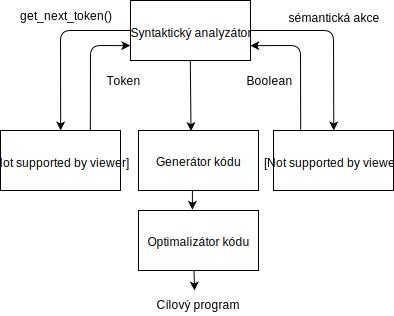
\includegraphics[width=0.7\textwidth, angle=0]{src/assets/structure.pdf}
\end{figure}

V následující části bude každá část interpretu posána podrobněji.
	\subsection{Lexikální analýza}
\label{subsec:lexer}
Úlohou Lexikálního analyzátoru je rozpoznávat jazykové lexémy a reprezentovat
je jako tokeny.

Lexikální analyzátor je implementací deterministického konečného
automatu. Jediný nedeterministický případ nastává tehdy, když má automat načítat znak ve tvaru $\backslash$\emph{ddd}.
Případ je vyřešen implementací interního čítače počtu načtených číslic. Pokud čítač dosáhne hodnoty 3 a načtená hodnota je
v~intervalu $\langle 001 - 255\rangle$, je znak úspěšné načten, v~opačném případě je ohlášena chyba v~lexikální
analýze.

Lexikální analyzátor je rozdělen do tří modulů: \ic|lexer.c|, \ic|lexer_fsm.c| a \ic|token.c|
. Modul \ic|token.c| obsahuje implementaci abstraktního datového typu token. Modul \ic|lexer_fsm.c|
obsahuje implementaci \textbf{deterministického konečného automatu}. Automat je oddělen od samotné implementace řízení lexikální analýzy z~důvodu snažšího testování veškerých přechodových stavů automatu mezi jednotlivými konfiguracemi. Modul \ic|lexer.c| poskytuje funkci
\ic|lexer_next_token|, která řídí činnost deterministického konečného automatu a vrací další token. Chyba v~lexikální analýze je rozpoznána \emph{navrácením tokenu s~příznakem chyby}.

\begin{figure}[htbp]
    \label{subsec:automat}
    \caption{Grafická reprezentace konečného automatu}
    \centering
    \includegraphics[width=0.9\textwidth, angle=0]{src/assets/automat.pdf}
\end{figure}

\subsection{Synataktická analýza}
Syntaxí řízený překlad je naimplementován v~modulu \ic|parser.c|, pro syntaktickou analýzu programu jako takového je
použita SA shoda dolů, konkrétně metoda \emph{rekurzivního sestupu}. Pro každé pravidlo z~LL gramatiky existuje v~tomto
modulu funkce realizující toto pravidlo.

Pro snažší zápis v~jazyce C byl implementován \textbf{poloautomatický systém generování funkcí pravidel} za pomocí maker.
Makra konkrétní pravidlo vykonají a zkontrolují jeho návratovou hodnotu, resp. úspěch kontroly. Pro kontrolu přítomnosti terminálu bylo
naimplemntováno makro \ic|CHECK_TOKEN(TOKEN_TYPE)|, pro spuštění jiného pravidla poté najri
\ic|CALL_RULE(NAME_OF_RULE)|.

Pro podmínečná volání pravidel makro
\ic|CHECK_RULE(type==TOKEN_TYPE,| \ic|NAME_OF_RULE,| \ic|REWIND_AND_SUCCESS)| - při jeho použití se spustí pravidlo
\ic|NAME_OF_RULE| v~případě, že je následující token typu \ic|TOKEN_TYPE| a jestliže bylo úspěšné, další načtený
token navrátí zpět lexikálnímu analyzátoru a prohlásí se volání za úspěšné.

Všechny pravidla pracují nad strukturou \ic|Parser|, která zapouzdřuje základní komponenty pro syntaxí řízený překlad.
Jedná se především od struktury \ic!ParserSemantic!, \ic!CodeConstructor! a \ic!Lexer!. První zmíněná zajištuje sémantické
kontroly programu; uchovává \emph{registr symbolů}, dočasné proměnné, pravidla pro implicitní konverze datových typů či
aktuální scénář SA, o~dalších kapitolách pojednávají jiné kapitoly. Po splnění některých pravidlech se v~SA vyskytují volání konstrukce kódu, kde je využito rozhraní z~modulu \ic!CodeConstructor! - SA tedy \textbf{není přímo zodpovědná za výslednou podobu cílového kódu}.

Některé derivace neterninálu \ic|<statement_single>| nemohou v~určitém kontextu nastat
- např. příkaz \ic|return| v~hlavním bloku programu. Syntaktická analýza si v~tomto případě \uv{vypomáhá} \textbf{sémantickými akcemi}, ačkoliv by tento problém mohla řešit sama. Takto upravená gramatika by se velmi rozrostla, což by snížilo její čitelnost.

Pro analýzu výrazů není analýza shora dolů v~případě jazyka \ic!IFJ17! možná, proto byla
použita standardní metoda zdola nahoru, v~našem případě založená na precedenční
syntaktické analýze - implementovaná v~modulu \ic|parser_expr.c|.

V~případě že je jako neterminál očekáván výraz, je volána funkce \ic|parser_parse_expr| ze zmíněného modulu, která provede \textbf{precedenční syntaktickou analýzu} výrazu a opět, jako ostatní pravidla, navrátí příznak úspěchu. V~rámci zpracování výrazů pomocí PA je také přímo generován cílový kód pomocí rozhraní modulu \ic|CodeGenerator|.

Neterminál \ic|<eols>| slouží ke \uv{zkonzumování} všech přebytečných znaků nového řádku - resp. terminálu \ic!EOL!. Jedná se o~univerzální neterminál použitý pro všechny možné výskyty většího množství znaků konců řádků. Proto je pro všechny terminály (kromě samotného \ic|EOL|) tohoto použito pravidlo \emph{60}.

\subsubsection{Gramatika a LL tabulka}
\begin{normalsize}
    \begin{enumerate}
        {\small
        \item <prog> $\rightarrow$ <body> <eols> EOF
        \item <body> $\rightarrow$ <definitions\_block> <scope> <shared\_variables\_declarations>

        \item <definitions\_block> $\rightarrow$ <eols> <definitions>

        \item <definitions> $\rightarrow$ <definition> <definitions\_block>
        \item <definitions> $\rightarrow$ $\varepsilon$

        \item <definition> $\rightarrow$ <function\_declaration>
        \item <definition> $\rightarrow$ <function\_definition>
        \item <definition> $\rightarrow$ <shared\_variable\_declaration>

        \item <function\_definition> $\rightarrow$ <function\_header> EOL <eols> <statements> END FUNCTION EOL
        \item <function\_declaration> $\rightarrow$ DECLARE <function\_header> EOL

        \item <function\_header> $\rightarrow$ FUNCTION IDENTIFIER (<function\_params>) AS <type> EOL

        \item <function\_params> $\rightarrow$ $\varepsilon$
        \item <function\_params> $\rightarrow$ <function\_param> <function\_n\_param>

        \item <function\_n\_param> $\rightarrow$ $\varepsilon$
        \item <function\_n\_param> $\rightarrow$ , <function\_param> <function\_n\_param>

        \item <function\_param> $\rightarrow$ IDENTIFIER AS <type>


        \item <type> $\rightarrow$ INTEGER
        \item <type> $\rightarrow$ BOOLEAN
        \item <type> $\rightarrow$ STRING
        \item <type> $\rightarrow$ DOUBLE

        \item <statements> $\rightarrow$ $\varepsilon$
        \item <statements> $\rightarrow$ <statement\_single> EOL <eols> <statements>


        \item <statement\_single> $\rightarrow$ <identifier\_assignment>
        \item <statement\_single> $\rightarrow$ <input>
        \item <statement\_single> $\rightarrow$ <return>
        \item <statement\_single> $\rightarrow$ <print>
        \item <statement\_single> $\rightarrow$ <condition>
        \item <statement\_single> $\rightarrow$ <while\_>
        \item <statement\_single> $\rightarrow$ <variable\_declaration>
        \item <statement\_single> $\rightarrow$ <static\_variable\_declaration>
        \item <statement\_single> $\rightarrow$ <scope>

        \item <variable\_declaration> $\rightarrow$ DIM IDENTIFIER AS <type> <declaration\_assignment>
        \item <declaration\_assignment> $\rightarrow$ E
        \item <declaration\_assignment> $\rightarrow$ <assignment>

        \item <shared\_variables\_declarations> $\rightarrow$ E
        \item <shared\_variables\_declarations> $\rightarrow$ <shared\_variable\_declaration>
        \item <shared\_variable\_declaration> $\rightarrow$ DIM SHARED IDENTIFIER AS <type> <declaration\_assignment>

        \item <static\_variable\_declaration> $\rightarrow$ STATIC IDENTIFIER AS <type> <declaration\_assignment>

        \item <return> $\rightarrow$ RETURN <expr>

        \item <assignment> $\rightarrow$ = <expression>
        \item <assignment> $\rightarrow$ <modify> <expression>
        \item <modify> $\rightarrow$ +=
        \item <modify> $\rightarrow$ -=
        \item <modify> $\rightarrow$ *=
        \item <modify> $\rightarrow$ /=
        \item <modify> $\rightarrow$ $\backslash$=

        \item <print> $\rightarrow$ PRINT <print\_expression> <print\_expressions>
        \item <print\_expressions> $\rightarrow$ E
        \item <print\_expressions> $\rightarrow$ <print\_expression> <print\_expressions>
        \item <print\_expression> $\rightarrow$ <expression> SEMICOLON

        \item <while\_> $\rightarrow$ DO WHILE <expression> EOL <eols> <cycle\_statements> LOOP

        \item <input> $\rightarrow$ INPUT IDENTIFIER

        \item <identifier\_assignment> $\rightarrow$  IDENTIF <assignment>

        \item <condition> $\rightarrow$ IF <expr> THEN EOL <eols> <statements> <condition\_elseif> <condition\_else> END IF
        \item <condition\_elseif> $\rightarrow$ $\varepsilon$
        \item <condition\_elseif> $\rightarrow$ ELSEIF <expr> THEN EOL <eols> <statements> <condition\_elseif>

        \item <condition\_else> $\rightarrow$ $\varepsilon$
        \item <condition\_else> $\rightarrow$ ELSE EOL <eols> <statements>

        \item <eols> $\rightarrow$ $\varepsilon$
        \item <eols> $\rightarrow$ EOL <eols>
        }
        \newpage
        \begin{landscape}
            \begin{table}[htbp]
                \label{table:prec}
                \centering
                \caption{LL tabulka 1. část}
                \begin{tabular}{|l|l|l|l|l|l|l|l|l|l|l|l|l|l|l|l|l|l|l|l|l|l|l|l|l|}
                    \hline
                    & {\rotatebox[origin=c]{90}{Operátor}}  & ( & ) & {\rotatebox[origin=c]{90}{identifier}}
                    & {\rotatebox[origin=c]{90}{integer literal}} & = & ; & {\rotatebox[origin=c]{90}{as}}
                    & {\rotatebox[origin=c]{90}{asc}}

                    & {\rotatebox[origin=c]{90}{delcare}} & {\rotatebox[origin=c]{90}{dim}}
                    & {\rotatebox[origin=c]{90}{do}} & {\rotatebox[origin=c]{90}{double}}
                    & {\rotatebox[origin=c]{90}{else}} & {\rotatebox[origin=c]{90}{end}}
                    & {\rotatebox[origin=c]{90}{chr}} & {\rotatebox[origin=c]{90}{function}}

                    & {\rotatebox[origin=c]{90}{if}} & {\rotatebox[origin=c]{90}{input}}
                    & {\rotatebox[origin=c]{90}{integer}} & {\rotatebox[origin=c]{90}{length}}
                    & {\rotatebox[origin=c]{90}{loop}} & {\rotatebox[origin=c]{90}{print}}
                    & {\rotatebox[origin=c]{90}{return}}
                    \\ \hline

                    <prog>&&&&&&&&&&1&&&&&&&1&&&&&&&
                    \\ \hline
                    <body>&&&&&&&&&&2&&&&&&&2&&&&&&&
                    \\ \hline
                    <def\_b>&&&&&&&&&&3&&&&&&&3&&&&&&&
                    \\ \hline
                    <defs>&&&&&&&&&&4&&&&&&&4&&&&&&&
                    \\ \hline
                    <def>&&&&&&&&&&6&&&&&&&7&&&&&&&
                    \\ \hline
                    <f\_def>&&&&&&&&&&&&&&&&&9&&&&&&&
                    \\ \hline
                    <f\_he>&&&&&&&&&&&&&&&&&10&&&&&&&
                    \\ \hline
                    <f\_pas>&&&12&13&&&&&&&&&&&&&&&&&&&&
                    \\ \hline
                    <f\_n\_p>&&&14&15&&&&&&&&&&&&&&&&&&&&
                    \\ \hline
                    <f\_pa>&&&&16&&&&&&&&&&&&&&&&&&&&
                    \\ \hline
                    <type>&&&&&&&&&&&&&20&&&&&&&17&&&&
                    \\ \hline
                    <sts>&&&&&&&&&&&&&&&21&&&&&&&&&
                    \\ \hline
                    <stsi>&&&23&&&&&&&&29&28&&&&&&27&24&&&&26&25
                    \\ \hline
                    <va\_de>&&&&&&&&&&&32&&&&&&&&&&&&&
                    \\ \hline
                    <va\_as>&&&&&&34&&&&&32&&&&&&&&&&&&&
                    \\ \hline
                    <s\_v\_ds>&&&&&&&&&&35&36&&&&&&35&&&&&&&
                    \\ \hline
                    <st\_v\_d>&&&&&&&&&&35&36&&&&&&35&&&&&&&
                    \\ \hline
                    <ret>&&&&&&&&&&&&&&&&&&&&&&&&39
                    \\ \hline
                    <ass>&&&&&&40&&&&&&&&&&&&&&&&&&
                    \\ \hline
                    <mod>&&&&&&&&&&&&&&&&&&&&&&&&
                    \\ \hline
                    <pr>&&&&&&&&&&&&&&&&&&&&&&&47&
                    \\ \hline
                    <pr\_es>&49&49&49&&&&&&&&&&&&&&&&&&&&48&
                    \\ \hline
                    <pr\_e>&50&50&50&&&&&&&&&&&&&&&&&&&&&
                    \\ \hline
                    <while>&&&&&&&&&&&&51&&&&&&&&&&&&
                    \\ \hline
                    <input>&&&&&&&&&&&&&&&&&&&52&&&&&
                    \\ \hline
                    <id\_a>&&&&53&&&&&&&&&&&&&&&&&&&&
                    \\ \hline
                    <con>&&&&&&&&&&&&&&&&&&54&&&&&&
                    \\ \hline
                    <con\_ei>&&&&&&&&&&&&&&55&55&&&54&&&&&&
                    \\ \hline
                    <con\_e>&&&&&&&&&&&&&&58&57&&&&&&&&&
                    \\ \hline
                    <con\_eols>&59&59&59&59&59&59&59&59&59&59&59&59&59&59&59&59&59&59&59&59&59&59&59&59
                    \\ \hline
                \end{tabular}
            \end{table}
        \end{landscape}
        \newpage
        \begin{landscape}
            \begin{table}[htbp]
                \label{table:prec2}
                \centering
                \caption{LL tabulka 2. část}
                \begin{tabular}{|l|l|l|l|l|l|l|l|l|l|l|l|l|l|l|l|l|l|l|l|l|l|l|l|l|l|l|l|l|l|}
                    \hline


                    & {\rotatebox[origin=c]{90}{scope}}
                    & {\rotatebox[origin=c]{90}{string}} & {\rotatebox[origin=c]{90}{substr}}
                    & {\rotatebox[origin=c]{90}{then}} & {\rotatebox[origin=c]{90}{while}}
                    & {\rotatebox[origin=c]{90}{and}} & {\rotatebox[origin=c]{90}{boolean}}
                    & {\rotatebox[origin=c]{90}{continue}} & {\rotatebox[origin=c]{90}{elseif}}
                    & {\rotatebox[origin=c]{90}{exit}} & {\rotatebox[origin=c]{90}{false}}
                    & {\rotatebox[origin=c]{90}{for}} & {\rotatebox[origin=c]{90}{next}}
                    & {\rotatebox[origin=c]{90}{not}} & {\rotatebox[origin=c]{90}{or}}
                    & {\rotatebox[origin=c]{90}{shared}} & {\rotatebox[origin=c]{90}{static}}
                    & {\rotatebox[origin=c]{90}{true}} & {\rotatebox[origin=c]{90}{double literal}}
                    & {\rotatebox[origin=c]{90}{string value}} & {\rotatebox[origin=c]{90}{comma}}
                    & {\rotatebox[origin=c]{90}{EOL}}
                    & {\rotatebox[origin=c]{90}{error}} & {\rotatebox[origin=c]{90}{EOF}}
                    & {\rotatebox[origin=c]{90}{+=}} & {\rotatebox[origin=c]{90}{-=}}
                    & {\rotatebox[origin=c]{90}{*=}} & {\rotatebox[origin=c]{90}{/=}}
                    & {\rotatebox[origin=c]{90}{\textbackslash=}}
                    \\ \hline
                    <prog>&1&&&&&&&&&&&&&&&1&&&&&&1&&&&&&&
                    \\ \hline
                    <body>&2&&&&&&&&&&&&&&&2&&&&&&2&&&&&&&
                    \\ \hline
                    <def\_b>&3&&&&&&&&&&&&&&&3&&&&&&3&&&&&&&
                    \\ \hline
                    <defs>&5&&&&&&&&&&&&&&&4&&&&&&&&&&&&&
                    \\ \hline
                    <def>&5&&&&&&&&&&&&&&&8&&&&&&&&&&&&&
                    \\ \hline
                    <f\_def>&&&&&&&&&&&&&&&&&&&&&&&&&&&&&
                    \\ \hline
                    <f\_he>&&&&&&&&&&&&&&&&&&&&&&&&&&&&&
                    \\ \hline
                    <f\_pas>&&&&&&&&&&&&&&&&&&&&&&&&&&&&&
                    \\ \hline
                    <f\_n\_p>&&&&&&&&&&&&&&&&&&&&&&&&&&&&&
                    \\ \hline
                    <f\_pa>&&&&&&&&&&&&&&&&&&&&&&&&&&&&&
                    \\ \hline
                    <type>&&19&&&&&18&&&&&&&&&&&&&&&&&&&&&&
                    \\ \hline
                    <sts>&&&&&&&&&&&&&&&&&&&&&&&&&&&&&
                    \\ \hline
                    <va\_de>&&&&&&&&&&&&&&&&&&&&&&&&&&&&&
                    \\ \hline
                    <va\_as>&&&&&&&&&&&&&&&&&&&&&&33&&&&&&&
                    \\ \hline
                    <s\_v\_ds>&1&&&&&&&&&&&&&&&&&&&&&&&&&&&&
                    \\ \hline
                    <st\_v\_d>&&&&&&&&&&&&&&&&&38&&&&&&&&&&&&
                    \\ \hline
                    <ret>&&&&&&&&&&&&&&&&&&&&&&&&&&&&&
                    \\ \hline
                    <ass>&&&&&&&&&&&&&&&&&&&&&&&&&41&41&41&41&41
                    \\ \hline
                    <mod>&&&&&&&&&&&&&&&&&&&&&&&&&42&43&44&45&46
                    \\ \hline
                    <pr>&&&&&&&&&&&&&&&&&&&&&&&&&&&&&
                    \\ \hline
                    <pr\_es>&&&49&&&&&&&&&&&&&&&&&&&48&&&&&&&
                    \\ \hline
                    <pr\_e>&&&50&&&&&&&&&&&&&&&&&&&&&&&&&&
                    \\ \hline
                    <while>&&&&&&&&&&&&&&&&&&&&&&&&&&&&&
                    \\ \hline
                    <input>&&&&&&&&&&&&&&&&&&&&&&&&&&&&&
                    \\ \hline
                    <id\_a>&&&&&&&&&&&&&&&&&&&&&&&&&&&&&
                    \\ \hline
                    <con>&&&&&&&&&&&&&&&&&&&&&&&&&&&&&
                    \\ \hline
                    <con\_ei>&&&&&&&&&56&&&&&&&&&&&&&&&&&&&&
                    \\ \hline
                    <con\_e>&&&&&&&&&&&&&&&&&&&&&&&&&&&&&
                    \\ \hline
                    <con\_eols>&59&59&59&59&59&59&59&59&59&59&59&59&59&59&59&59&59&59&59&59&59&60&59&59&59&59&59&59&59

                    \\ \hline
                \end{tabular}

            \end{table}
        \end{landscape}
        \newpage
    \end{enumerate}
\end{normalsize}
\subsubsection{Precedenční analýza výrazů}

Precedenční analýza je řízena precedenční tabulkou, kterou se vyhodnocuje pořadí zpracování tokenů.
. V~tabulce se nachází jak \textbf{binární, tak i unární mínus}. Lexikální analyzátor nám ovšem poskytuje pouze jeden token mínus a proto se unární a binární mínus musí vyhodnotit \textbf{podle kontextu}.

Precedenční analýza využívá \textbf{zásobník v~podobě obousměrně vázaného seznamu}, do kterého se ukládají terminály,precedenční symboly a neterminály. Pomocí redukčních pravidel, která jsou vypsána v~příloze, je výraz postupně redukován.
Vzhledem k~tomu, že je překladač založen na přímém překladu, je při redukování pomocí pravidel přímo voláno generování kódu, resp. v~případech konstatních literálů je \textbf{výraz rovnou vyhodnocován}, viz kapitola \ref{subsec:optimization-cee}.

\begin{table}[!htbp]
    \centering
    \label{tabul:prav}
    \caption{Redukční pravidla}
    \begin{tabular}{lll}
        $E \to i$ & $E \to E - E$ & $E \to E >= E$\\
        $E \to (E)$ & $E \to E ~ / ~ E$ & $E \to E < E$\\
        $E \to i()$ & $E \to E ~ \backslash ~ E$ & $E \to E <= E$\\
        $E \to i(E)$ & $E \to - E$ & $E \to NOT ~ E$\\
        $E \to i(E, E)$ & $E \to E = E$ & $E \to E ~ AND ~ E$\\
        $E \to i(E, E, ...)$ & $E \to E <> E$ & $E \to E ~ OR ~ E$\\
        $E \to E + E$ & $E \to E > E$\\
    \end{tabular}
\end{table}

\begin{table}[htbp]
\label{tabul:prec}
\centering
\caption{Precedenční tabulka}
\label{precedencni-tabulka}
\begin{tabular}{|r|c|c|c|c|c|c|c|c|c|c|c|c|c|c|c|c|c|c|c|c|}
\hline
& $un -$ & $*$ & $/$ & $\backslash$ & $+$ & $-$ & $=$ & $<>$ & $<$ & $<=$ & $>=$ & $>$ & $NOT$ & $AND$ & $OR$ & $($ & $)$ & $,$ & $i$ & \$ \\ \hline
$un -$ &$<$&$>$&$>$&$>$&$>$&$>$&$>$&$>$&$>$&$>$&$>$&$>$& x &$>$&$>$&$<$&$>$&$>$&$<$&$>$\\ \hline
$*$ &$<$&$>$&$>$&$>$&$>$&$>$&$>$&$>$&$>$&$>$&$>$&$>$&$<$&$>$&$>$&$<$&$>$&$>$&$<$&$>$\\ \hline
$/$ &$<$&$>$&$>$&$>$&$>$&$>$&$>$&$>$&$>$&$>$&$>$&$>$&$<$&$>$&$>$&$<$&$>$&$>$&$<$&$>$\\ \hline
$\backslash$ &$<$&$<$&$<$&$>$&$>$&$>$&$>$&$>$&$>$&$>$&$>$&$>$&$<$&$>$&$>$&$<$&$>$&$>$&$<$&$>$\\ \hline
$+$ &$<$&$<$&$<$&$<$&$>$&$>$&$>$&$>$&$>$&$>$&$>$&$>$&$<$&$>$&$>$&$<$&$>$&$>$&$<$&$>$\\ \hline
$-$ &$<$&$<$&$<$&$<$&$>$&$>$&$>$&$>$&$>$&$>$&$>$&$>$&$<$&$>$&$>$&$<$&$>$&$>$&$<$&$>$\\ \hline
$=$ &$<$&$<$&$<$&$<$&$<$&$<$& x & x & x & x & x & x &$<$&$>$&$>$&$<$&$>$&$>$&$<$&$>$\\ \hline
$<>$ &$<$&$<$&$<$&$<$&$<$&$<$& x & x & x & x & x & x &$<$&$>$&$>$&$<$&$>$&$>$&$<$&$>$\\ \hline
$<$ &$<$&$<$&$<$&$<$&$<$&$<$& x & x & x & x & x & x &$<$&$>$&$>$&$<$&$>$&$>$&$<$&$>$\\ \hline
$<=$ &$<$&$<$&$<$&$<$&$<$&$<$& x & x & x & x & x & x &$<$&$>$&$>$&$<$&$>$&$>$&$<$&$>$\\ \hline
$>=$ &$<$&$<$&$<$&$<$&$<$&$<$& x & x & x & x & x & x &$<$&$>$&$>$&$<$&$>$&$>$&$<$&$>$\\ \hline
$>$ &$<$&$<$&$<$&$<$&$<$&$<$& x & x & x & x & x & x &$<$&$>$&$>$&$<$&$>$&$>$&$<$&$>$\\ \hline
$NOT$ & x &$>$&$>$&$>$&$>$&$>$&$>$&$>$&$>$&$>$&$>$&$>$&$<$&$>$&$>$&$<$&$>$&$>$&$<$&$>$\\ \hline
$AND$ &$<$&$<$&$<$&$<$&$<$&$<$&$<$&$<$&$<$&$<$&$<$&$<$&$<$&$>$&$>$&$<$&$>$&$>$&$<$&$>$\\ \hline
$OR$ &$<$&$<$&$<$&$<$&$<$&$<$&$<$&$<$&$<$&$<$&$<$&$<$&$<$&$<$&$>$&$<$&$>$&$>$&$<$&$>$\\ \hline
$($ &$<$&$<$&$<$&$<$&$<$&$<$&$<$&$<$&$<$&$<$&$<$&$<$&$<$&$<$&$<$&$<$& = & = &$<$& x \\ \hline
$)$ &$>$&$>$&$>$&$>$&$>$&$>$&$>$&$>$&$>$&$>$&$>$&$>$&$>$&$>$&$>$& x &$>$&$>$& x &$>$\\ \hline
$,$ &$<$&$<$&$<$&$<$&$<$&$<$&$<$&$<$&$<$&$<$&$<$&$<$&$<$&$<$&$<$&$<$& = & = &$<$& x \\ \hline
$i$ & x &$>$&$>$&$>$&$>$&$>$&$>$&$>$&$>$&$>$&$>$&$>$& x &$>$&$>$& = &$>$&$>$& x &$>$\\ \hline
\$ &$<$&$<$&$<$&$<$&$<$&$<$&$<$&$<$&$<$&$<$&$<$&$<$&$<$&$<$&$<$&$<$& x & x &$<$& x\\ \hline
\end{tabular}
\end{table}


\subsection{Sémantická analýza}
Sémantické kontroly jsou přidruženy k~syntaktickým pravidlům v~rekurzivním sestupu a
precedenční syntaktické analýze výrazů. Jsou organizovány do tzv. \textbf{scénářů}. Jeden scénář
sémanticky popisuje související část kódu. - např. definici
či deklaraci funkce. Sémantická analýza nám také pomáhá hlídat i některé \textbf{gramatické aspekty},
které by byly pro LL gramatiku příliš kompikované, nebo by měly příliš dlouhý zápis.

\subsection{Konstruktor kódu}
\label{subsec:code-constructor}
Konstruktor cílového kódu je komponenta překladače, který hlídá význam a odpovědnosti vygenerovaného tříadresného kódu \ic!IFJcode17!. Drží informace o~\textbf{vygenerovaných návěštích pro podmínky, cykly i funkce}, příznak generování kódu do bloku cyklu/vně, registr instrukcí pro konverze datových typů a další.

\subsection{Generátor cílového kódu}
Generátor kódu je nízkoúrovňová komponenta zastřešující skládání, validaci a vykreslování cílového kódu \ic|IFJcode17|.
Kontroluje generované instrukce a její operandy, tedy \textbf{validní kombinace typů operandů} (přístupy do rámců, konstatní
literály, návěští či datové typy) u~konkrétních instrukcí.

Interní implementace spoléhá na \emph{obousměrně svázaný lineární seznam} struktur \ic|CodeInstruction|, které kromě
režijních ukazatelů uchovávají typ instrukce a ukazatele na až tři operandy, struktury \ic|CodeInstructionOperand|.
Tento seznam je uložen v~datové struktuře \ic|CodeGenerator|, která dále obsahuje pole podpisů\footnote{Podpis
instrukce je složena z~bitových masek definující povolené typy operandů a její textové reprezentace v~kódu} \ic!IFJcode17!. instrukcí pro jejich validace.
Struktura \ic|CodeInstructionOperand| uchovává informace o~svém typu a poté unii dat pro konkrétní typ operandu, tedy
ukazatel na proměnnou \ic|SymbolVariable|,
data konstanty \ic|CodeInstructionOperandConstantData| v~unii s~datovým typem nebo řetězec uchovávající název návěští.

\subsection{Optimalizátor kódu}
Následující blok obsahuje výčet implementovaných optimalizačních procesů - ty jsou spoušteny v~našimi experimenty zjištěném pořadí a některé i mnohonásobně s~různou konfigurací - vždy tak, aby nedošlo k~funkčně neekvivalentním úpravám programu. 

\begin{description}
    \item[Značkování hotového cílového kódu] Protože jsme nebyli schopni jednoznačně určit, zda daná instrukce patří do těla funkce, či je součásti výrazu, byla zvolena metoda označení instrukcí již při \emph{syntaktické analýze}, kde je možno určit instrukce, které se vygenerovaly v~rámci určitého pravidla např. výrazu.
    
    \item[Vyhodnocování konstatních výrazů v~PA]\label{subsec:optimization-cee} Optimalizace pracuje již při redukci výrazu pomocí \emph{precedenční syntaktické analýzy}, v~jednotlivých pravidlech se zjišťuje, zda jsou dané \textbf{výrazy konstantní literály} a pokud ano, tak se místo generování diskrétních instrukcí pro vyhodnocení generuje instrukce pro přímé vložení již vyhodnocené hodnoty na základě konstatních literálů. Tato optimalizace tedy jako jediná \textbf{nepracuje s~instrukcemi} jazyka \ic|IFJcode17|.
    
    \item[Odstranění nepoužitých symbolů] Před odstraněním nepoužitých symbolů, se nejdříve \textbf{provede analýza} nagenerovaného \ic|IFJcode17| kódu, kde se vytvoří \emph{tabulka s~rozptýlenými položkami}, kde klíč je unikátní identifikátor symbolu a hodnota je počet použití z~daného symbolu. Avšak přestože je \ic|READ| instrukce zápisu, má věnjší vliv, tudíž inkrementujeme počet použití symbolu. Ostatní instrukce zápisu včetně \ic|DEFVAR| se nepoučítají jako použití proměnné. Následně jsou odstraněny všechny nepoužité funkce a proměnné včetně jejich výrazy do nich zapisující.
    
    \item[Optimalizace \uv{peephole}] Tato optimalizace pracuje nad malými segmenty vygenerovaného kódu. Pracuje tak, že nalezne sekvenci instrukcí, které odpovídají určitému \textbf{vzoru} a následně danou sekvenci \textbf{nahradí efektivnější} (ce se týče ceny \ic|IFJcode17|) sekvencí instrukcí. Tuto optimalizaci jsme navíc rozšířili o~podmíněnost počtu výskytů symbolů, které se mohou objevit v~operandech. Bohužel tato optimalizace může odstranit značky instrukcí, v~prvním běhu jsou použita \uv{mírnější pravidla}, narozdíl od toho druhého, který zároveň porušuje značky.
    
    \item[Interpretace celých konstantních výrazů] Při aktualizaci statistikách o~instrukcích se také zjistí, zda výrazy obsahují pouze literálové operandy a až jednu pomocnou proměnnou, která je používána pro přetypování hodnoty pod vrcholem zásobníku. Jestliže je obsah intepretovatelný, je poté provedena \emph{interpretace}, kterou zapouzdřuje struktura \ic|Interpreter|. Tento interpreter interpretuje \textbf{pouze zásobníkové instrukce}. Toto omezení jsme si mohli dovolit z~důvodu, že všechny výrazy jsou generovány pouze pomocí zásobníkových instrukcí.
    
    \item[Částečná interpretace] Narozdíl od \emph{interpretace celých konstantních výrazů} tato optimalizace pracuje s~co nejmenší možnou interpretovatelnou \emph{sekvencí instrukcí}. Proto tato optimalizace nepracuje s~příznaky instrukcí, ale pouze hledá předem zadanou sekvencí instrukcí, kterou je schopna interpretovat a nahradit na vložení instrukce s~vypočtenou hodnotou.
    
    \item[Šíření konstant] Algoritmus této optimalizace byl ze všech výše zmíněných nejkomplikovanější. Nejdříve je nutno jednotlivé instrukce rozdělit do bloků, které jsou uzly \emph{orientovaného grafu}. Následně se zjistí \emph{silně propojené komponenty}, které označují cykly, či rekurzi a naleznou se všechny proměnné, které byly v~daných blocích modifikovány, tyto proměnné budou vyřazeny při šíření konstant v~daných blocích. Při šíření konstant je použit \emph{zásobník tabulek konstant}. \\Blok, který je spojen s~předchozím blokem podmíněnou hranou např. podmínka, je použita nejvyšší tabulka na zásobníku, která je označená příznakem, že daná tabulka byla vytvořena v~předchozím bloku a do daného bloku vedla přímá hrana. Jestliže je do bloku lze dostat přímým skokem, je použita tabulka z~vrcholu zásobníku a daná tabulka se označí příznakem. \\Po zpracování bloku a všech bloků, do kterých vedla z~daného bloku hrana, je \textbf{vyjmuta} z~vrcholu zásobníku tabulka konstant, která odpovídá tabulce, která byla vytvořena v~daném bloku. Kvůli možnosti funkcí ovlivňovat globální proměnné, jsou \textbf{funkce odříznuté od uzlů} hlavního programu. Následně se začíná šíření konstant ve funkcích s~prázdnými tabulkami, čímž se docílí izolovaného šíření konstant ve funkcích.
\end{description}

\newpage
\section{Rozšíření}
\begin{multicols}{2}

\subsection{SCOPE}
Pro implementaci tohoto rozšíření byla upravena tabulka symbolů na \textbf{zásobníkovou strukturu tabulek} tak, aby byla schopna reagovat vložením/výjmutím na základě průchodu zdrojovým programem.
Takto je možno dosáhnout až potenciálně nekonečné hloubky \textbf{zanoření bloků bez konfliktních symbolů proměnných} - tuto strukturu jsme pracovně nazvali \ic!SymbolRegister! - rozhraní této struktury poté volají konkrétní sémantické akce.

Definici proměnné v~bloku cyklu je poté problém pro konstruktor kódu, který příšlušnou instrukci definující nový symbol umístí před tělo cyklu.

\subsection{GLOBAL}
Rozšíření GLOBAL bylo implementováno v~gramatice přidáním
nových \textbf{pravidel pro definici statických a globálních proměnných}.
Dále byla upraven registr symbolů (jak je popsáno pro \ic|SCOPE|),
ve kterém je nejnižší tabulka vyhrazena
pro globální proměnné. Názvy statických proměnných jsou zaprefixovány
jménem funkce a jsou uloženy v~globálním rámci cílového jazyka. 
\emph{Způsobem implementace by si kompilátor mohl dovolit i možnost inicializace statické proměné ve funkci \textbf{nestaticky} (např. parametrem), ale dle chování FREEBASIC bylo toto potlačeno.}

\subsection{UNARY}
Pro rozšíření UNARY byla implementována nová \textbf{gramatická pravidla} pro zkrácené přířazování - i sémantické akce odpovídají přiřazení, liší se pouze vygenerovaný kód. Unární mínus poté řeší \textbf{PA pomocí speciálního případu} při zpracování.

\subsection{BASE}
Rozšíření bylo implementuje LA - ta je schopna \textbf{rozpoznat
lexémy označující čísla ve dvojkové, osmičkové a šestnáctkové} soustavě a
výsledek převést na desítkové číslo, se kterým již nakládáno dále identicky jako původně s~desítkovým.

\subsection{FUNEXP}
Volání funkcí ve výrazech bylo implementováno na úrovni \textbf{precedenční syntaktické analýzy},
precedenční tabulka obsahuje redukční pravidla pro redukování funkcí, čímž implementuje i
možnost \textbf{libovolného volání funkcí} ve výrazech.

\subsection{IFTHEN}
Implementováno na gramatické úrovni přidáním \textbf{nepovinných částí}
\ic!elseif! a odstraněních povinnosti mít část \ic!else!.
Konstruktor kódu poté používá \textbf{zásobník návěští} pro skoky mezi jednotlivými bloky podmínky.

\subsection{BOOLOP}
Precedenční tabulka byla modifikována, aby podporovala i logické operace \ic|AND|, \ic|OR| a \ic|NOT|.
Těmto operacím přísluší i sémantické akce \textbf{kontrolující povolené datové typy} a konstruování kódu (které je velmi obdobné s~kódem pro matematické operace).

\end{multicols}
	\section{Použité algorimy a datové structury}
\subsection{Tabulka symbolů}
Pro implementaci tabulky symbolů jsme zvolili hashovací
tabulku.
\todo{Pepo, prosím o pár vět}

\begin{figure}[htbp]
    \centering
    \includegraphics[width=0.6\textwidth, angle=0]{src/assets/symbol_table.pdf}
\end{figure}

\subsection{Správa paměti}
\todo{Sony, dopiš to prosím, nerozumím tomu. Jen pár vět :D}

	\section{Práce v týmu}
\todo{Write something about our team work}
	\section{Závěr}
Úlohou projektu bylo především si vykoušet techniky přednášené v~předmětech IFJ a IAL prakticky,
naučit se metody výstavby překladačů, získat další znalosti z~programování v~týmu a také vzájemnou spolupráci.

Projekt byl pro nás velkou \textbf{výzvou} a svou odborností převyšoval vše, s~čím jsme do té doby měli dočinění - práce na projektu nám přinesla velké množství zkušeností.

Kromě správnosti jsme se také zaměřovali na \textbf{správnou dekompozici} problémů a snahu o~\uv{čistý} kód. Výsledný překladač je obohacen o~7 rozšíření a byl vyvíjen dle normy \emph{C11}, je tedy nezávislý na platformě. Repozitář tohoto projektu bude po domluvě zveřejněn na serveru GitHub\footnote{Projekt bude po termínu odevzdání zveřejněn na adrese \href{https://github.com/thejoeejoee/IFJ-VUT-BIT-2017-2018/}{https://github.com/thejoeejoee/IFJ-VUT-BIT-2017-2018/}.}.

Z implementace optimalizací nám vyvstanuly některé problémy týkající se kompilace - z těch méně významných jde především o spotřebu paměti - i u jednoduchých programů se jedná o \textbf{desítky MB požadované paměti}. Vyhodnocováním konstatních výrazů jsme také narazili na problém přesnosti předávání operandů v jazyce \ic|IFJcode17| do interpretu tohoto jazyka - řešili jsme v kooperaci s zadávajícími, kteří nám vyhověli a upravili \ic|IFJcode17| pro příjem operandů typu \ic|float| s vyšší přesností.

\emph{
	Z~metrik projektu by bylo vhodné zmínit počet majoritních souborů, 40 .c, 40 .h a 25 .cpp jednotkových testů, celkem \emph{24805} řádků zdrojového kódu a \emph{903} commitů v~systému \emph{Git}, průměrně \emph{10} denně za aktivní dny vývoje.
}

\vfill
\section{Použitá literatura, software a služby}

\renewcommand\labelenumi{[\arabic{enumi}]}
\renewcommand\theenumi\labelenumi
\begin{enumerate}
%literatura
	\item Alexander Meduna a Roman Lukáš, \emph{Formální jazyky a
překladače}, podklady k přednáškám, 17. září 2017

	\item Anurag Singh, \uv{Tarjan’s Algorithm to find Strongly Connected Components}, \emph{GeeksforGeeks}, získáno 22. listopadu 2017 z \href{http://www.geeksforgeeks.org/tarjan-algorithm-find-strongly-connected-components/}{http://www.geeksforgeeks.org/tarjan-algorithm-find-strongly-connected-components/}

	\item \emph{Optimizing compiler}, Wikipedia, získáno 20. listopadu 2017 z \href{https://en.wikipedia.org/wiki/Optimizing\_compiler}{https://en.wikipedia.org/wiki/Optimizing\_compiler}

	\item \emph{One-pass compiler}, Wikipedia, získáno 10. října 2017 z \href{https://en.wikipedia.org/wiki/One-pass\_compiler}{https://en.wikipedia.org/wiki/One-pass\_compiler}

	\item International Organization for Standardization, \emph{C standard ISO/IEC 9899:201x}, 2. prosinec 2010, \\\href{http://www.open-std.org/jtc1/sc22/wg14/www/docs/n1548.pdf}{http://www.open-std.org/jtc1/sc22/wg14/www/docs/n1548.pdf}

	\item cppreference.com, \emph{C and C++ reference}, 1. prosinec 2017, \href{http://en.cppreference.com/}{http://en.cppreference.com/}
\end{enumerate}

\renewcommand\labelenumi{[\Alph{enumi}]}
\renewcommand\theenumi\labelenumi
\vspace{20pt}
\begin{enumerate}
	\item  Josef Kolář a Son Hai Nguyen, \emph{Advánc IFJcode17 IDE}, 1.4.10, 3. prosinec 2017,\\\href{https://github.com/thejoeejoee/VUT-FIT-IFJ-2017-toolkit}{https://github.com/thejoeejoee/VUT-FIT-IFJ-2017-toolkit}
	\item JetBrains s.r.o., CLion, 2017.3, 30. listopad 2017, \href{https://www.jetbrains.com/clion/}{https://www.jetbrains.com/clion/}
	\item The Qt Company, Qt Creator IDE, 4.4.1, 6. říjen 2017, \href{https://www.qt.io/qt-features-libraries-apis-tools-and-ide/\#ide}{https://www.qt.io/qt-features-libraries-apis-tools-and-ide/\#ide}
	\item Microsoft Corporation, Visual Studio Community 2017, 15.4.3, 8. listopad 2017,\\\href{https://www.visualstudio.com/cs/vs/community/}{https://www.visualstudio.com/cs/vs/community/}
	\item GNU Project, \emph{GCC}, 5.4, 3. červen 2016, \href{https://gcc.gnu.org/}{https://gcc.gnu.org/}
	\item MinGW Project, \emph{MinGW}, 5.0.3, 4. listopad 2017, \href{http://mingw.org/}{http://mingw.org/}
	\item Junio Hamano and others, \emph{Git}, 2.15.1, 28. listopad 2017, \href{https://git-scm.com/}{https://git-scm.com/}
\end{enumerate}

\renewcommand\labelenumi{[\Roman{enumi}]}
\renewcommand\theenumi\labelenumi
\vspace{20pt}
\begin{enumerate}
	\item GitHub, Inc, \emph{GitHub}, 2017, \href{https://github.com/}{https://github.com/}
	\item Codecov, \emph{Codecov}, 2017, \href{https://codecov.io/}{https://codecov.io/}
	\item Travis CI, GmbH, \emph{Travis CI}, 2017, \href{https://travis-ci.com/}{https://travis-ci.com/}
\end{enumerate}
	\newpage	
	\section{Předpřipravené ukázky}

Pokud je váš počítač chráněný firewallem nebo proxy serverem, zkontrolujte, že má Firefox povolený přístup k internetu.
\todo{Todo section}

\subsection{Pseudokod algoritmu}

\begin{algorithm}[h]
    \For{$i = 0$ \KwTo $100$}{
    print\_number = true\;
    \If{i is divisible by 3}{
    print\_number = false\;
    }
    \If{i is divisible by 5}{
    print "Buzz"\;
    }
    print a newline\;
    }
    \caption{Ukázka pseudokodu algoritmu}
\end{algorithm}

\subsection{Kod v programovacím jazyce}

\begin{lstlisting}[caption = Print arguments of command line]
#include <stdio.h>

/**
* Comments are gray but it can by styled by configure values in dokumentace.tex
*
* @param int argc Count of arguments of command line
* @param *char[] argv List of command line arguments
*/
int main(int argc, char *argv[]) {

// For cycle
for(int i = 0; i < argc; i++) {
printf("%s\n", argv[i]);
}
return 0;
}
\end{lstlisting}
\subsection{Vizualizace datových struktur}
\includesvg{src/assets/data_structure}
	\newpage
Redukční pravidla\\

{\large
$E \to i$\\
$E \to (E)$\\
$E \to i()$\\
$E \to i(E)$\\
$E \to i(E, E)$\\
$E \to i(E, E, ...)$\\
$E \to E + E$\\
$E \to E - E$\\
$E \to E ~ / ~ E$\\
$E \to E ~ \backslash ~ E$\\
$E \to - E$\\
$E \to E = E$\\
$E \to E <> E$\\
$E \to E > E$\\
$E \to E >= E$\\
$E \to E < E$\\
$E \to E <= E$\\
$E \to NOT ~ E$\\
$E \to E ~ AND ~ E$\\
$E \to E ~ OR ~ E$\\
}
	\subsection{Precedenční analýza}
Precedenční analýza se využívá při zpracovávání výrazů. Pokud syntaktická analýza najde pravidlo pro zpracování výrazu, přenechá ho právě jí. Precedenční analýza je řízena precedenční tabulkou, kterou se vyhodnocuje pořadí zpracování tokenů. Tato tabulka je k nalezení v příloze.
\todo{Move text to proper location}



\begin{table}[]
\centering
\caption{Precedenční tabulka}
\label{precedencni-tabulka}
\begin{tabular}{|l|l|l|l|l|l|l|l|l|l|l|l|l|l|l|l|l|l|l|l|l|}
\hline
 & $un -$ & $*$ & $/$ & $\backslash$ & $+$ & $-$ & $=$ & $<>$ & $<$ & $<=$ & $>=$ & $>$ & $NOT$ & $AND$ & $OR$ & $($ & $)$ & $,$ & $i$ & \$ \\ \hline
$un -$ &$<$&$>$&$>$&$>$&$>$&$>$&$>$&$>$&$>$&$>$&$>$&$>$& x &$>$&$>$&$<$&$>$& x &$<$&$>$\\ \hline
$*$ &$<$&$>$&$>$&$>$&$>$&$>$&$>$&$>$&$>$&$>$&$>$&$>$&$<$&$>$&$>$&$<$&$>$&$>$&$<$&$>$\\ \hline
$/$ &$<$&$>$&$>$&$>$&$>$&$>$&$>$&$>$&$>$&$>$&$>$&$>$&$<$&$>$&$>$&$<$&$>$&$>$&$<$&$>$\\ \hline
$\backslash$ &$<$&$<$&$<$&$>$&$>$&$>$&$>$&$>$&$>$&$>$&$>$&$>$&$<$&$>$&$>$&$<$&$>$&$>$&$<$&$>$\\ \hline
$+$ &$<$&$<$&$<$&$<$&$>$&$>$&$>$&$>$&$>$&$>$&$>$&$>$&$<$&$>$&$>$&$<$&$>$&$>$&$<$&$>$\\ \hline
$-$ &$<$&$<$&$<$&$<$&$>$&$>$&$>$&$>$&$>$&$>$&$>$&$>$&$<$&$>$&$>$&$<$&$>$&$>$&$<$&$>$\\ \hline
$=$ &$<$&$<$&$<$&$<$&$<$&$<$&$>$&$>$&$>$&$>$&$>$&$>$&$<$&$>$&$>$&$<$&$>$&$>$&$<$&$>$\\ \hline
$<>$ &$<$&$<$&$<$&$<$&$<$&$<$&$>$&$>$&$>$&$>$&$>$&$>$&$<$&$>$&$>$&$<$&$>$&$>$&$<$&$>$\\ \hline
$<$ &$<$&$<$&$<$&$<$&$<$&$<$&$>$&$>$&$>$&$>$&$>$&$>$&$<$&$>$&$>$&$<$&$>$&$>$&$<$&$>$\\ \hline
$<=$ &$<$&$<$&$<$&$<$&$<$&$<$&$>$&$>$&$>$&$>$&$>$&$>$&$<$&$>$&$>$&$<$&$>$&$>$&$<$&$>$\\ \hline
$>=$ &$<$&$<$&$<$&$<$&$<$&$<$&$>$&$>$&$>$&$>$&$>$&$>$&$<$&$>$&$>$&$<$&$>$&$>$&$<$&$>$\\ \hline
$>$ &$<$&$<$&$<$&$<$&$<$&$<$&$>$&$>$&$>$&$>$&$>$&$>$&$<$&$>$&$>$&$<$&$>$&$>$&$<$&$>$\\ \hline
$NOT$ & x &$>$&$>$&$>$&$>$&$>$&$>$&$>$&$>$&$>$&$>$&$>$&$<$&$>$&$>$&$<$&$>$& x &$<$&$>$\\ \hline
$AND$ &$<$&$<$&$<$&$<$&$<$&$<$&$<$&$<$&$<$&$<$&$<$&$<$&$<$&$>$&$>$&$<$&$>$&$>$&$<$&$>$\\ \hline
$OR$ &$<$&$<$&$<$&$<$&$<$&$<$&$<$&$<$&$<$&$<$&$<$&$<$&$<$&$<$&$>$&$<$&$>$&$>$&$<$&$>$\\ \hline
$($ &$<$&$<$&$<$&$<$&$<$&$<$&$<$&$<$&$<$&$<$&$<$&$<$&$<$&$<$&$<$&$<$& = & = &$<$& x \\ \hline
$)$ &$>$&$>$&$>$&$>$&$>$&$>$&$>$&$>$&$>$&$>$&$>$&$>$&$>$&$>$&$>$& x &$>$&$>$& x &$>$\\ \hline
$,$ &$<$&$<$&$<$&$<$&$<$&$<$&$<$&$<$&$<$&$<$&$<$&$<$&$<$&$<$&$<$&$<$& = & = &$<$& x \\ \hline
$i$ & x &$>$&$>$&$>$&$>$&$>$&$>$&$>$&$>$&$>$&$>$&$>$& x &$>$&$>$& = &$>$&$>$& x &$>$\\ \hline
\$ &$<$&$<$&$<$&$<$&$<$&$<$&$<$&$<$&$<$&$<$&$<$&$<$&$<$&$<$&$<$&$<$& x & x &$<$& x\\ \hline
\end{tabular}
\end{table}

\end{document}